\section{Проблематика выбора объектов}
\begin{frame}{C чем мы имеем дело?}
	%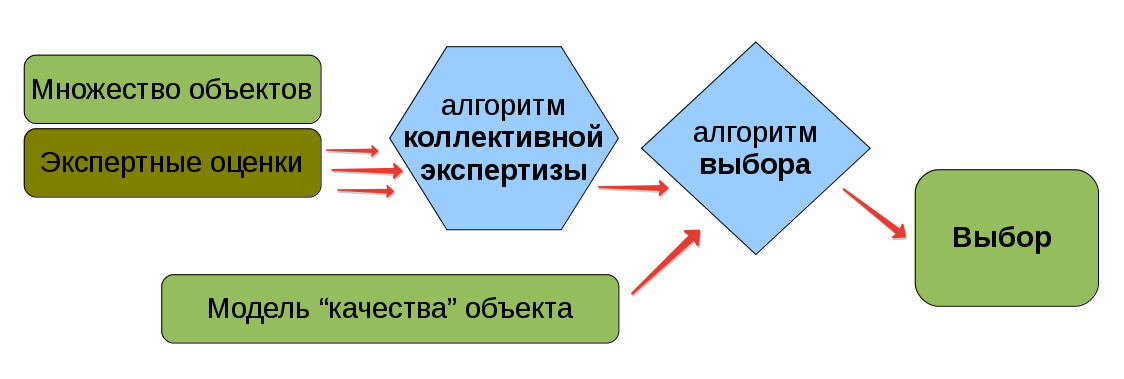
\includegraphics[width=0.8\linewidth]{./pic/globalscheme}
 	\begin{columns}
 		\column{0.50\textwidth}
 			Есть $n$ объектов, у каждого объекта % составителем методологии выбрано
 			есть $m$ нечётких параметров: 
			\\ \vspace*{2mm}
 			$\tilde x_{ij} \in X$, {\footnotesize $i = 1 \ldots n$, $j = 1 \ldots m$} 
 			\\ \vspace*{3mm}
 			$x_{ij} \in X$ -- их значения (неизвестны), где $X$ --  числовое множество. %некое выпуклое подмножество действительной оси
 		\column{0.50\textwidth}
 			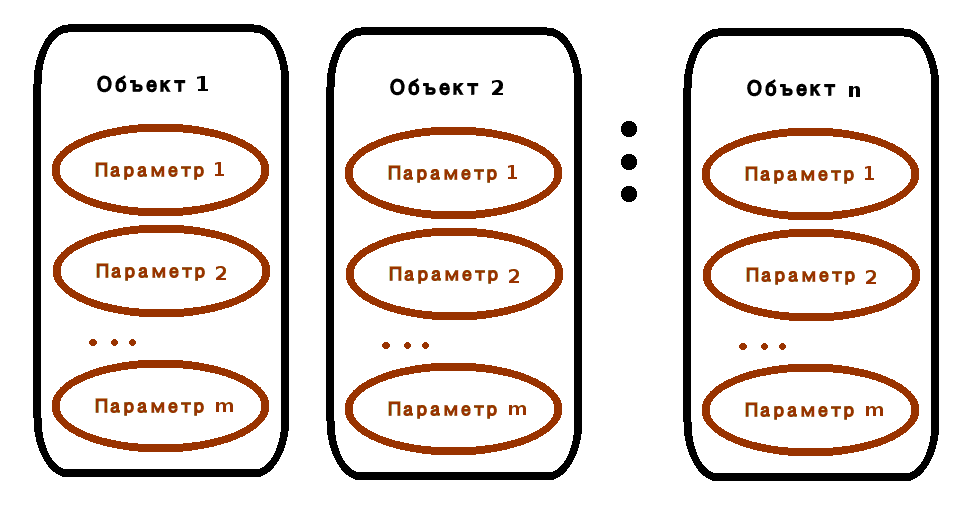
\includegraphics[width=1.0\linewidth]{./pic/theobjects}
 	\end{columns}
 	
        \hspace{20mm} { \small \tikz { \node  (n1) { \light{монотонна и задана заказчиком экспертизы}  }; } }
	 $x_i = \tikz[baseline] { \node[anchor=base, fill=green!20] (t1) {$f$}; } (x_{i1}, ..., x_{im})$ -- <<качество>> объектов.
	\begin{tikzpicture}[overlay]
		\path[->] (n1.west) edge  (t1.north east);
	\end{tikzpicture}

	\vspace*{3mm}
	\begin{columns}
		\column{0.60\textwidth}
		Экспертные оценки -- это распределения 
		{\large \begin{center} \hspace{-20mm}  $\{ \p_{ij}(x_{ij}) \}^{(r)}$ \end{center} }
		{\footnotesize где $i = 1 \ldots n$ -- номер объекта, $j = 1 \ldots m$, -- номер параметра, $r = 1 \ldots R$ -- номер эксперта}.  
		\column{0.40\textwidth}
		\begin{center}
			\vspace*{-8mm}
			%   {\small Примеры оценок:}
			  {\scriptsize {Примеры оценок: значения $\p(x)$ показаны цветом, $x \in \setTen$}}
			  \\ \vspace*{2mm}
			  \resizebox{1.0\linewidth}{!}{\showevDisplayFullScale{./pic/chapter01-tech01.dat}}
		\end{center}
	\end{columns}
 \end{frame} %===========================

\begin{frame}{Пример модели <<качества>> объекта}
	\begin{center}
		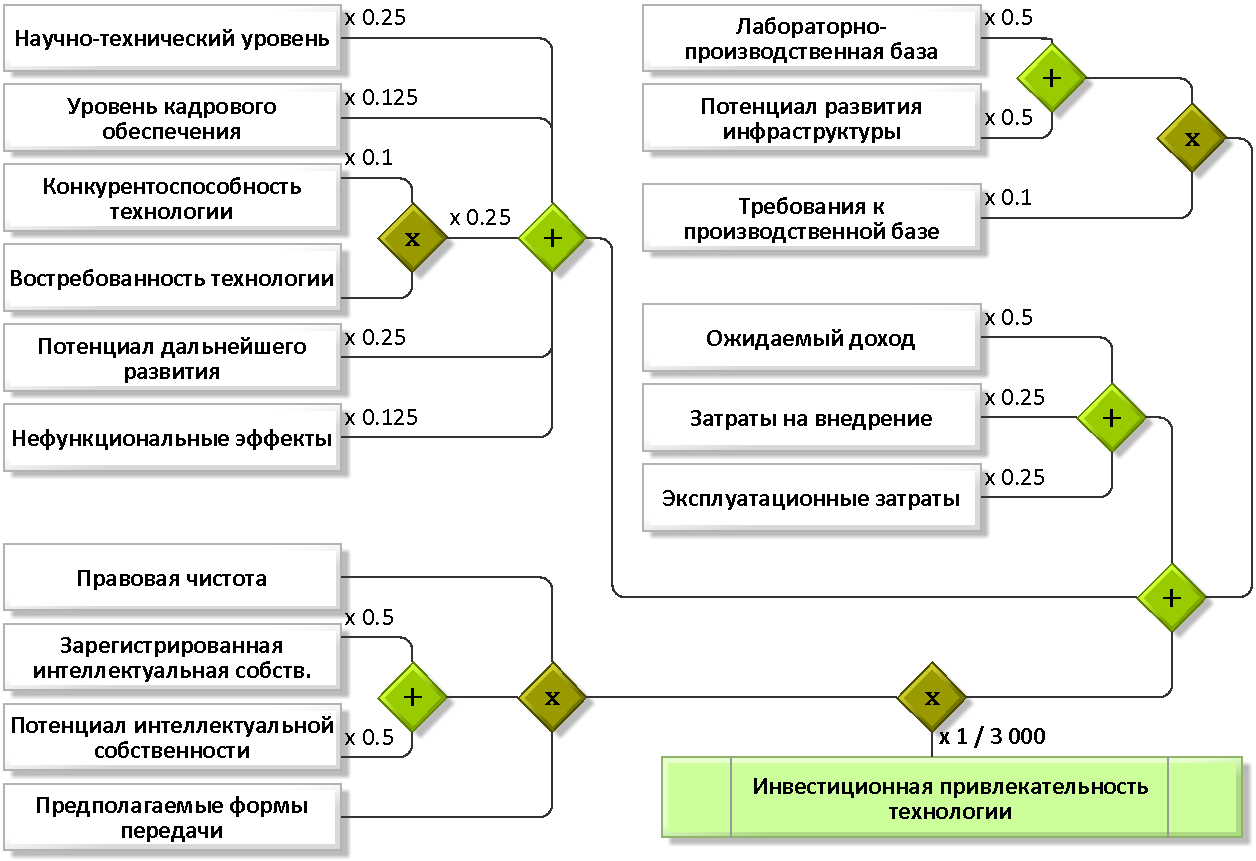
\includegraphics[width=0.9\linewidth]{./pic/schemeF2}
	\end{center}
\end{frame} %===========================

\section{Задача и алгоритм выбора}
\begin{frame}{Основная задача выбора объектов}
	%\begin{center}
	\hspace*{0.125\linewidth}
	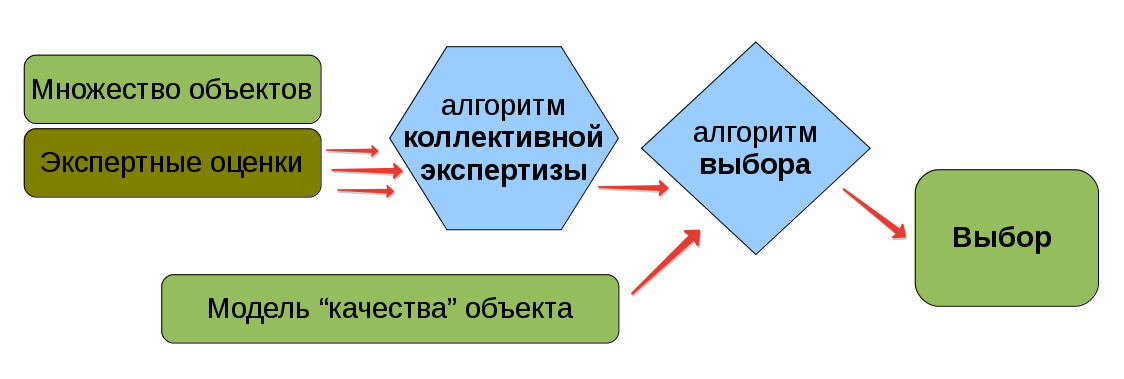
\includegraphics[width=0.75\linewidth]{./pic/globalscheme}
	%\end{center}
	\\ Для задачи выбора эксперт \emph{один} (или результат коллективной экспертизы), $\{\p_{ij}\}$ -- его оценки,
	{\footnotesize $i = 1 \ldots n$, $j = 1 \ldots m$}. Они порождают $ \OAP$:
	\\ \vspace*{2mm} $ \Om = \{\theta = t\},\; \theta = (\tilde x_{11}, ..., \tilde x_{nm}) \text{ -- вектор всех параметров всех объектов} $.
	\\ \vspace*{2mm} Пусть $d \subset \setN$ -- какое-то решение, $\delta_t$ -- верное решение: %нсли бы знали x_i
	\begin{gather*}
	      \delta_{t} \define= \{i_1, \mydots, i_k\}: \forall\, i \in \delta_t,\; \forall\, i' \in \setN \setminus \delta_t: x_i > x_{i'},
	      \\ {\footnotesize \text{если бы мы знали } x_i = f(x_{i1}, ..., x_{im})  \forall i \in \setN.}
	 \end{gather*}
	  \vspace*{-8mm}
	\begin{center}
	      \vspace*{1mm}
	     Задача: \tikz[baseline] {  \node[anchor=base, fill=green!20]{ $\P(\{d \neq \delta_t\}) \sim \underset{d} \min$ }; },
	     где $\abs{d} = \abs{\delta_t} = k$ -- наперёд задано. % размер подможества.
	\end{center}
\end{frame} %===========================

\begin{frame}{Алгоритм выбора: работа с  возможностью}
\begin{gather*}
	\text{\small Возьмем любое событие $A$, в частности, $A= \{d \neq \delta_t\}$.}
	\\ \P(A) > p_0 \in \zo \text{?.. Решается легко из-за свойств $\sup$ и $\inf$.}
	\\ \hspace*{4mm} {\small  t \define= (x_{11}, \ldots, x_{nm}) \text{ -- вектор значений всех параметров всех объектов.} }
\end{gather*}
{\large 
  \hspace{6mm} $\P($\tikz[baseline]{\node[anchor=base, fill=green!20](nPA){$A$};}$\displaystyle  ) = \sup_{ t \in A}\;\inf_{i, j}\,\p_{ij}(x_{ij})\; $
  \hspace{8mm} \tikz[baseline]{\node[anchor=base, fill=green!20](nB){$B$};}$ \define= \{t:  \forall i,j\; \p_{ij}(x_{ij}) > p_0\}$
}
\begin{center}
    \tikz{ \node (tSets) { 
\includegraphics[width=0.5\linewidth]{./pic/algo_sets_simple} };}
    \\ Наш алгоритм за время $O(nm)$ позволяет проверить, пересекаются ли $A= \{d \neq \delta_t\}$ и $B$. Если и только если пересекаются, $\P(\{d \neq \delta_t\}) > p_0$.
\end{center}
\begin{tikzpicture}[overlay]
	\path[->] (nPA.south) edge [bend right] (tSets.west);
	\path[->] (nB.south) edge (tSets.north north east);
\end{tikzpicture}
\end{frame}

% == eof == eof ===